\section{Programmation}

\begin{frame}
    \frametitle{Programmation}
    \begin{figure}[H]
        \centering
        \begin{minipage}{.5\textwidth}
            \centering
            Le robot, équipé des cartes designées, ne peut rien faire sans code. Cette partie a été étudiée en cours de PT1 et nous sera utile pour programmer le robot en C.
        \end{minipage}%
        \begin{minipage}{.5\textwidth}
            \centering
            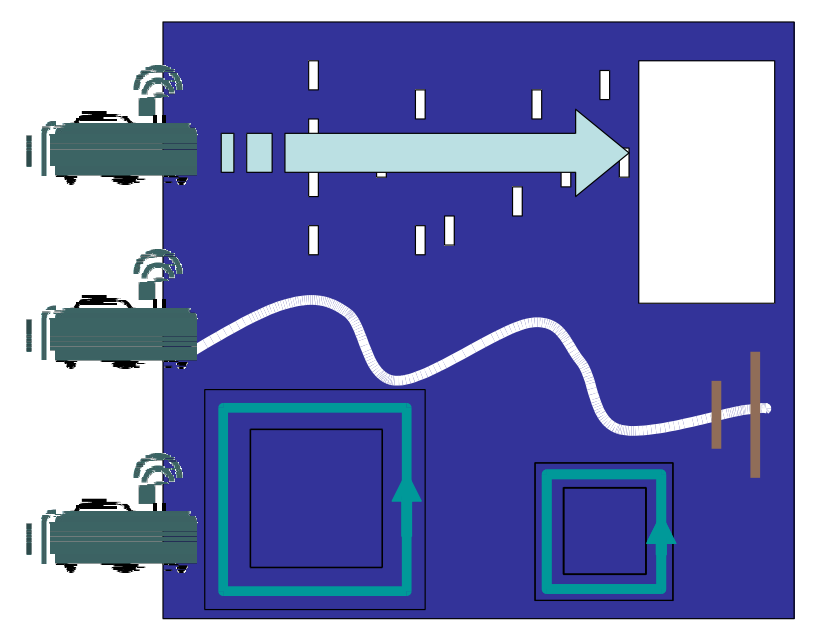
\includegraphics[width=.7\linewidth]{Images/programmes.png}
            \caption{Les trois démonstrations}
            \label{fig:programmes}
        \end{minipage}%
    \end{figure}

\footer{\hfill\insertframenumber/\inserttotalframenumber}
\end{frame}

\begin{frame}[fragile]
\frametitle{Le code}
\begin{lstlisting}[language=C, caption=Lecture des données capteur (vu en PT1)]
int main(void) {
  while(true){
    // Lecture des valeurs des capteurs de ligne
    double leftSensor1Value = leftLineSensor1.read();
    double leftSensor2Value = leftLineSensor2.read();
    double rightSensor1Value = rightLineSensor1.read();
    double rightSensor2Value = rightLineSensor2.read();
  }
}
\end{lstlisting}

\footer{\hfill\insertframenumber/\inserttotalframenumber}
\end{frame}